\section{Theoretical Approach}
%
Experimental coincidence spectra are given by the multitude of
kinetic energies $E_{\rm sec}$ of the secondary electron
and the intensities of the peaks. The latter is proportional to the
probability of the decay as well as the theoretically determinable
decay width $\Gamma=\frac{\hbar}{\tau}$,
which is inverse proportional to the lifetime $\tau$ of the decay process.
The manifold of the
secondary energies and decay widths will therefore compose the electron-electron
coincidence spectrum.
In case of noble gas clusters
with given geometrical structures three aspects have to be taken into account:
different decay mechanisms, the possibility to decay with multiple
interaction partners and different decay channels $\beta$ within
each decay mechanism.
At the current stage of development we need to neglect the nuclear dynamics which
additionally might play an important role.

%We are interested in describing the electron emission spectra of excited states in clusters, that where measured by the electron-electron coincidence method in our experiments. 
%In our theoretical description, these will be composed of multiple transitions, each characterized by a kinetic energy $E_{\rm sec}$ of the secondary electrons, and the intensity of the peak.
%The latter is proportional to the probability of the decay, represented here by the decay width $\Gamma_\beta = \hbar/\tau_\beta$, where $\tau_\beta$ is the lifetime due to the respective transition.
%The total decay width $\Gamma$ is the sum of all partial $\Gamma_\beta$.
%In case of noble gas clusters with a given geometrical structure, three aspects have to be taken into account:
%different decay mechanisms, the contribution of different cluster sites to the respective decay, and the existence of different decay channels within each decay mechanism.
%At the current stage of development we have to neglect the nuclear dynamics, which

This means, for the evaluation of the decay width we are dealing with a sum over three different indices: 
For a given structure it is most convenient to
start with a decomposition of the system into interaction partners of
the different, relevant decay mechanisms, i.e. pairs (combination of two atoms regardless
of their internuclear distance) for the ICD and triples (combinations of three atoms)
for the ETMD3.
These atoms do not necessarily need to form bonds between each other or
even be close, but they are characterized according to fixed internal
coordinates. 
Each pair and each triple leads to a decay spectrum that can be described by the energy of the secondary electron and the decay width, which is in first order of approximation independent of other atoms present in the cluster.
In the following, this approach will be called model of pairs and triples.


%Decomposing every system into pairs and triples of atoms is a very useful
%first order approximation to both the investigation of energies and
%decay widths of a larger system. Pairs and triples are combinations of
%two and three atoms, respectively.

In order to determine, whether a channel $\beta$ for a given geometry and decay
mechanism is open, i.e., whether it is in accordance with energy conservation,
knowledge of the energies of the initial and the final states, $E_{\rm in}$ and $E_{\rm fin}$, of
the corresponding processes are necessary.
If the channel
is open, the excess energy is carried away by the emitted electron
in form of its kinetic energy $E_{\rm sec}$. These energies in the model
of pairs and triples can be approximated by

\begin{align}
 E_{\rm in}        &= SIP(X_{\rm in}) \label{equation:E_in}\\
 E_{\rm fin}^\beta &= SIP(X_{D}^\beta) + SIP(X_{E}^\beta) + \frac 1d
           \label{equation:E_fin}\\
 E_{\rm sec}^\beta &= E_{\rm in}^\beta - E_{\rm fin}^\beta \label{equation:E_sec}
\end{align}
where $X_{\rm in}$ denotes the initially ionized atom and
$X_{D}$ and $X_{E}$ describe the electron donating atom and electron
emitting atom, respectively.
$\beta$ denotes the decay channel characterized by the quantum numbers of the ionized atoms in the pairs and triples, $SIP(X^\beta)$ the single ionization potential of vacancy $\beta$ in atom $X$ and $d$ the interatomic distance between the atoms $X_{D}$ and $X_{E}$. 
Atomic units are used.
The initially ionized atom $X_{\rm in}$ can
coincide with one or both of
the final state atoms
$X_{D}$ and $X_{E}$.
The distribution of the vacancies over the different
atoms determines the kind of electronic decay process at hand. Hence, in an
Auger process all three atoms coincide, for an ICD process $X_{\rm in}$
coincides with $X_{D}$, for an ETMD2 process $X_D$ and $X_E$ coincide
and for an {ETMD}3 process
all ionized states are located on different atoms.

\begin{figure}[h]
 \centering
 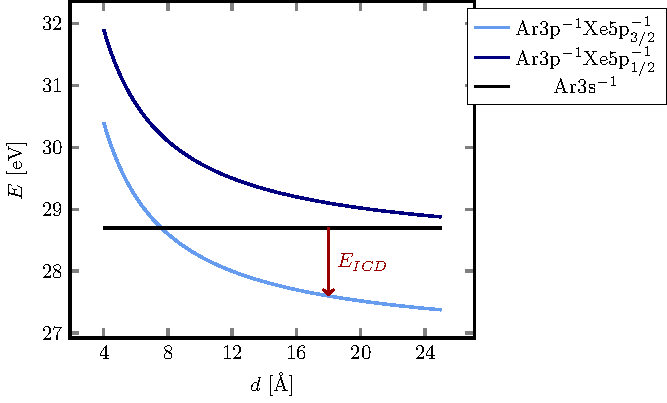
\includegraphics[width=8.5cm]{pics/channel_open_ICD.pdf}
 \caption{Initial (black trace) and final state energies (blue traces) 
          for ICD in ArXe pairs as a function of 
          internuclear distance, using the experimental ionization potentials given
          in Table \ref{tab:valence}. For distances larger than the channel opening
          distance the ICD channel is open.}
 \label{figure:channel_open_ICD}
\end{figure}

The electron emitted by autoionization has the kinetic energy $E_{\rm sec}$. 
If the calculated value of $E_{\rm sec}$ is negative,
the final state energy is higher than the initial state energy and the        
process is energetically not accessible. Hence, the corresponding channel     
is closed, as shown in Figure \ref{figure:channel_open_ICD}. Related to
the opening of each channel is an internuclear distance which we will call 
\emph{channel opening distance} in the following.
                                                               
This {\latin ad hoc} approach allows to easily correct for energetic shifts of ionization potentials as observed in larger clusters by adding experimentally or theoretically determined energy shifts $\Delta E(X_{I}^{\beta})$ for a given vacancy $I={\rm in},D,E$ and channel $\beta$. This yields the working expression for the kinetic energy of the secondary electron:

\begin{equation}
 E_{\rm sec}^\beta = SIP(X_{\rm in}) + \Delta E (X_{\rm in})
               - SIP(X_{D}^\beta) - \Delta E (X_{D}^\beta)
               - SIP(X_{E}^\beta) - \Delta E (X_{E}^\beta)
               - \frac 1d .
\end{equation}

The total decay width $\Gamma$ is given by the sum over the decay widths
of all decay mechanisms. In case of the ArXe clusters we only consider
ICD and ETMD3, because the ETMD2 pathway is energetically not accessible:

\begin{equation}
 \Gamma = \Gamma_{\rm ICD} + \Gamma_{\rm ETMD} .
\end{equation}

These are given by the sum over the decay widths of all pairs $i$ for the
ICD and all triples $j$ for the ETMD(3), respectively, and over all channels $\beta$:
%
\begin{align}
 \Gamma_{\rm ICD}  &= \sum\limits_{i,\beta} N_{{\rm ICD},i}  \, \Gamma_{{\rm ICD},i,\beta},\\
 \Gamma_{\rm ETMD} &= \sum\limits_{j,\beta} N_{{\rm ETMD},j} \, \Gamma_{{\rm ETMD},j,\beta}.
\end{align}
Here, $N_{{\rm ICD},i}$ and $N_{{\rm ETMD},j}$ denote the number of geometrically
equal pairs and triples in a given cluster structure. The total number of pairs
reads
$N_{{\rm ICD}} = N_{\rm in} \cdot N_{D/E} = N_{\rm Ar} \cdot N_{\rm Xe}
 = \sum\limits_i N_{{\rm ICD},i}$ and the number of triples is
$N_{{\rm ETMD}} = N_{\rm in} \cdot N_{D/E} (N_{D/E} - 1) = N_{\rm Ar} \cdot N_{\rm Xe} (N_{\rm Xe} - 1)
 = \sum\limits_j N_{{\rm ETMD},j}$.
The numbers of geometrically equivalent pairs $N_{{\rm ICD},i}$ and triples $N_{{\rm ETMD},j}$
strongly depend on the structure of the cluster. From these relationships
it can be seen that a higher xenon content in the cluster statistically
favours the ETMD(3) over the ICD.

In previous work \cite{Fasshauer13,Fasshauer_thesis} we have shown that
the decay width for a single pair or triple for a distinct channel $\beta$
following Wentzel \cite{Wentzel27}, Feshbach\cite{Feshbach58,Feshbach62}
and Fano,\cite{Fano61}
%
\begin{equation}
 \Gamma_{\beta}(E_{\rm res}) = 2\pi \left|
                           \braket{\Phi_{\rm in}| H_f |\chi_{\beta}}
                           \right|^2,
\end{equation}
%
can be approximated by its asymptotic behaviour
%
\begin{equation}
 \Gamma_{{\rm ICD},i,\beta} = (2J_{\rm in}+1)\, \frac{3c^4}{8\pi}\,
                        \sum\limits_{M_{in}'}
                        \left| \left(
                        \begin{array}{ccc}
                        J_A'  & 1        & J_A\\
                        -M_A' & M_A'-M_A & M_A
                        \end{array}\right) \right|^2
                        \frac{\sigma^{(X_E)}(\omega_{vp,\beta})}
                        {R_i^6 \, \omega_{vp,\beta}^4 \tau_{in,\beta}},
\end{equation}
%
where $J_A$, $J_A'$ and $M_A$, $M_A'$ denote the total angular momentum of the
initially ionized atom (which is the same as the electron doner atom) in the
initial and final state, respectively,
and
%
\begin{align}
 \Gamma_{{\rm ETMD},j,\beta} =& \frac{c}{\pi} \sum\limits_{m,M_{in,D'}}
                        \frac{\Theta_{m,k}(\alpha_j) \sigma^{(X_E)}(\omega_{vp,\beta})
                              \left| <\tilde{D}_{m,j,\beta}(M_{in,D'})>\right|^2}
                         {R_j^6 \omega_{vp,\beta}}\\
               =& \frac{c}{\pi R_j^6}
               \sum\limits_{M_{in,D'}}
               \left( \left| <\tilde{D}_{x,j,\beta} (M_{in,D'}) > \right|^2
                 (2+ \sin^2\alpha_j)
               + \left| <\tilde{D}_{z,j,\beta} (M_{in,D'}) > \right|^2
                 (1+\cos^2\alpha_j) \right) \nonumber \\
           & \times\, \frac{c\sigma^{(X_E)}(\omega_{vp,\beta})}{\omega_{vp,\beta}}
\end{align}
%
depending on 
experimental properties
of atoms, like the ionization cross sections
$\sigma^{(X_E)}(\omega_{vp,\beta})$, radiative lifetimes of the initially
ionized state $\tau_{in,\beta}$ and the excess energy transferred to the
emitting atom (the energy of the virtual photon) $\omega_{vp,\beta}$
and calculated dipole transition moments $\tilde{D}_{m,j,\beta}$, only.
Here, $\Theta_{m}(\alpha_j)$ is a function depending on the angle $\alpha_j$
of the triple and the direction of the dipole
transition moment $m$
(compare Ref. \cite{Fasshauer13}).

In this work we evaluate the secondary energies and decay widths with
the program HARDRoC \cite{HARDRoC,fasshauer2014} using the
experimental ionization energies of Table \ref{tab:valence}
and data from the literature given in Tables II and III.
This choice is identical to the one made in Reference \cite{Fasshauer13}.
